
%%%%%%%%%%%%%%%%%%%%%%%%%%%%%%%%%%%%%%%%%%%%%%%%%%
%         	LÉWOZ
%%%%%%%%%%%%%%%%%%%%%%%%%%%%%%%%%%%%%%%%%%%%%%%%%%

{\large \textbf{Léwoz}}

Rythme de référence du gwoka, il exprime la lutte.
Il existe deux façons d'exécuter le léwoz selon la région -- à savoir le léwoz de Grande-Terre et le \textit{léwoz in-dès-twas} (de Sainte-Rose).
\bigskip
\begin{quote}
{%
\parindent 0pt
\noindent
\ifx\preLilyPondExample \undefined
\else
  \expandafter\preLilyPondExample
\fi
\def\lilypondbook{}%
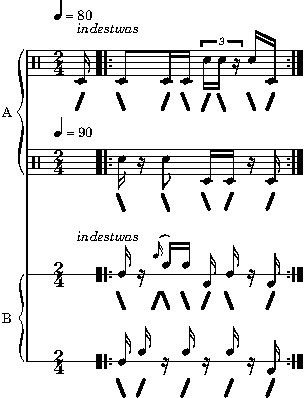
\includegraphics{87/lily-2de452d3-1}%
% eof

\ifx\postLilyPondExample \undefined
\else
  \expandafter\postLilyPondExample
\fi
}
\end{quote}


%%%%%%%%%%%%%%%%%%%%%%%%%%%%%%%%%%%%%%%%%%%%%%%%%%
%			PADJAMBEL
%%%%%%%%%%%%%%%%%%%%%%%%%%%%%%%%%%%%%%%%%%%%%%%%%%

\bigskip
\bigskip
{\large \textbf{Padjambel}}

Rythme de caractère guerrier au sens d'affranchissement à tout ce qui est avilissant.
\bigskip
\begin{quote}
{%
\parindent 0pt
\noindent
\ifx\preLilyPondExample \undefined
\else
  \expandafter\preLilyPondExample
\fi
\def\lilypondbook{}%
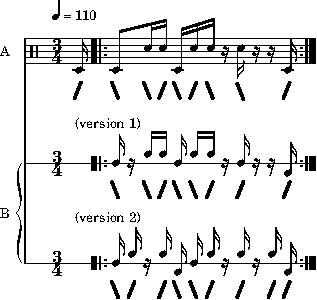
\includegraphics{82/lily-6d9f6c8a-1}%
% eof

\ifx\postLilyPondExample \undefined
\else
  \expandafter\postLilyPondExample
\fi
}
\end{quote}

%%%%%%%%%%%%%%%%%%%%%%%%%%%%%%%%%%%%%%%%%%%%%%%%%%
%			GRAJ
%%%%%%%%%%%%%%%%%%%%%%%%%%%%%%%%%%%%%%%%%%%%%%%%%%
\clearpage
\bigskip
\bigskip
{\large \textbf{Graj}}

Rythme de travail des champs.
\bigskip
\begin{quote}
{%
\parindent 0pt
\noindent
\ifx\preLilyPondExample \undefined
\else
  \expandafter\preLilyPondExample
\fi
\def\lilypondbook{}%
\includegraphics{4c/lily-56731605-1}%
% eof

\ifx\postLilyPondExample \undefined
\else
  \expandafter\postLilyPondExample
\fi
}
\end{quote}


%%%%%%%%%%%%%%%%%%%%%%%%%%%%%%%%%%%%%%%%%%%%%%%%%%
%			WOULÉ
%%%%%%%%%%%%%%%%%%%%%%%%%%%%%%%%%%%%%%%%%%%%%%%%%%
%\clearpage

\bigskip
\bigskip
{\large \textbf{Woulé}}

Rythme de travail.
\bigskip
\begin{quote}
{%
\parindent 0pt
\noindent
\ifx\preLilyPondExample \undefined
\else
  \expandafter\preLilyPondExample
\fi
\def\lilypondbook{}%
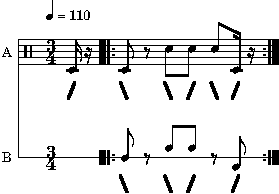
\includegraphics{89/lily-1a2b1a45-1}%
% eof

\ifx\postLilyPondExample \undefined
\else
  \expandafter\postLilyPondExample
\fi
}
\end{quote}

%%%%%%%%%%%%%%%%%%%%%%%%%%%%%%%%%%%%%%%%%%%%%%%%%%
%			KALADJA
%%%%%%%%%%%%%%%%%%%%%%%%%%%%%%%%%%%%%%%%%%%%%%%%%%
%\clearpage
\bigskip
\bigskip

{\large \textbf{Kaladja}}

Se joue lentement -- dans ce cas, ce rythme exprime la souffrance ou la peine -- ou rapidement à l'instar du Toumblack.
\bigskip
\begin{quote}
{%
\parindent 0pt
\noindent
\ifx\preLilyPondExample \undefined
\else
  \expandafter\preLilyPondExample
\fi
\def\lilypondbook{}%
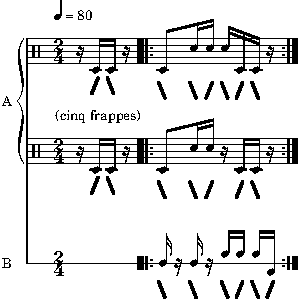
\includegraphics{a2/lily-64356649-1}%
% eof

\ifx\postLilyPondExample \undefined
\else
  \expandafter\postLilyPondExample
\fi
}
\end{quote}

%%%%%%%%%%%%%%%%%%%%%%%%%%%%%%%%%%%%%%%%%%%%%%%%%%
%			TOUMBLACK
%%%%%%%%%%%%%%%%%%%%%%%%%%%%%%%%%%%%%%%%%%%%%%%%%%
\bigskip
\bigskip
{\large \textbf{Toumblack}}

Rythme de fête dédié à la danse. Une partie du toumblack -- appelé \textit{tumblak chiré} -- consiste à accélérer le tempo jusqu'à l'ivresse, et se termine ainsi par une coda.
\bigskip
\begin{quote}
{%
\parindent 0pt
\noindent
\ifx\preLilyPondExample \undefined
\else
  \expandafter\preLilyPondExample
\fi
\def\lilypondbook{}%
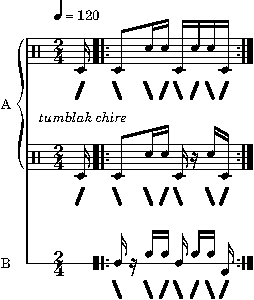
\includegraphics{7a/lily-a9c4e824-1}%
% eof

\ifx\postLilyPondExample \undefined
\else
  \expandafter\postLilyPondExample
\fi
}
\end{quote}


%%%%%%%%%%%%%%%%%%%%%%%%%%%%%%%%%%%%%%%%%%%%%%%%%%
%			MENDÈ
%%%%%%%%%%%%%%%%%%%%%%%%%%%%%%%%%%%%%%%%%%%%%%%%%%
%\clearpage

\bigskip
\bigskip
{\large \textbf{Mendè}}

Rythme de fête à caractère licencieux.
\bigskip
\begin{quote}
{%
\parindent 0pt
\noindent
\ifx\preLilyPondExample \undefined
\else
  \expandafter\preLilyPondExample
\fi
\def\lilypondbook{}%
\includegraphics{ad/lily-697ca8fb-1}%
% eof

\ifx\postLilyPondExample \undefined
\else
  \expandafter\postLilyPondExample
\fi
}
\end{quote}

%%%%%%%%%%%%%%%%%%%%%%%%%%%%%%%%%%%%%%%%%%%%%%%%%%

\bigskip
\bigskip
\par 
A - D'après Jean-Pierre \textsc{Solvet}, \textit{Solfège du tambour ka}. L'Harmattan, Paris 2007. 
\par
B - D'après \href{http://www.lameca.org}{LAMECA} - Médiathéque Caraïbe Dettino Lara, consulté en 2012. \\
%En ligne $\rightarrow$ \href{http://www.lameca.org/dossiers/gwoka/musique/rythmes/rythm.html}{\texttt{\footnotesize http://www.lameca.org/dossiers/gwoka/musique/rythmes/rythm.html}}
\par
* voir note \ref{ftn:konk} page \pageref{ftn:konk}.
%%%%%%%%%%%%%%%%%%%%%%%%%%%%%%%%%%%%%%%%%%%%%%%%%%
